The previous chapter described how to build a dataset which contains a collection of trajectories without taking into account different ship types. Since the original AIS records from AISHub do not include the static information of vessels, we had to crawl the openly accessible ship database \textit{myshiptracking.com}, fusing the MMSIs with their corresponding ship type as defined by the website. By analyzing the "all ships"-dataset and looking at the most encountered ship types in Fig. \ref{fig:shipTypes}, we notice a huge variety of different vessel models, ranging from big container ships and tankers to tugs, sailing- or fishing ships.

\begin{figure}[H]
    \centering
    \includesvg[width=0.95\textwidth]{images/shipTypes.svg}
    \caption{The 15 most encountered ship types in the dataset.}
    \label{fig:shipTypes}
\end{figure}

As already mentioned in subchapter \ref{subchap:curveEnv}, \cite{venskus2021unsupervised} construct separate computational models depending on the deviating ship types, as they found out that individual vessel types generate different traffic patterns (p.~729). We adhere to this idea and will assemble multiple datasets depending on different ship categories.
\begin{wrapfigure}{l}{0.5\textwidth}
    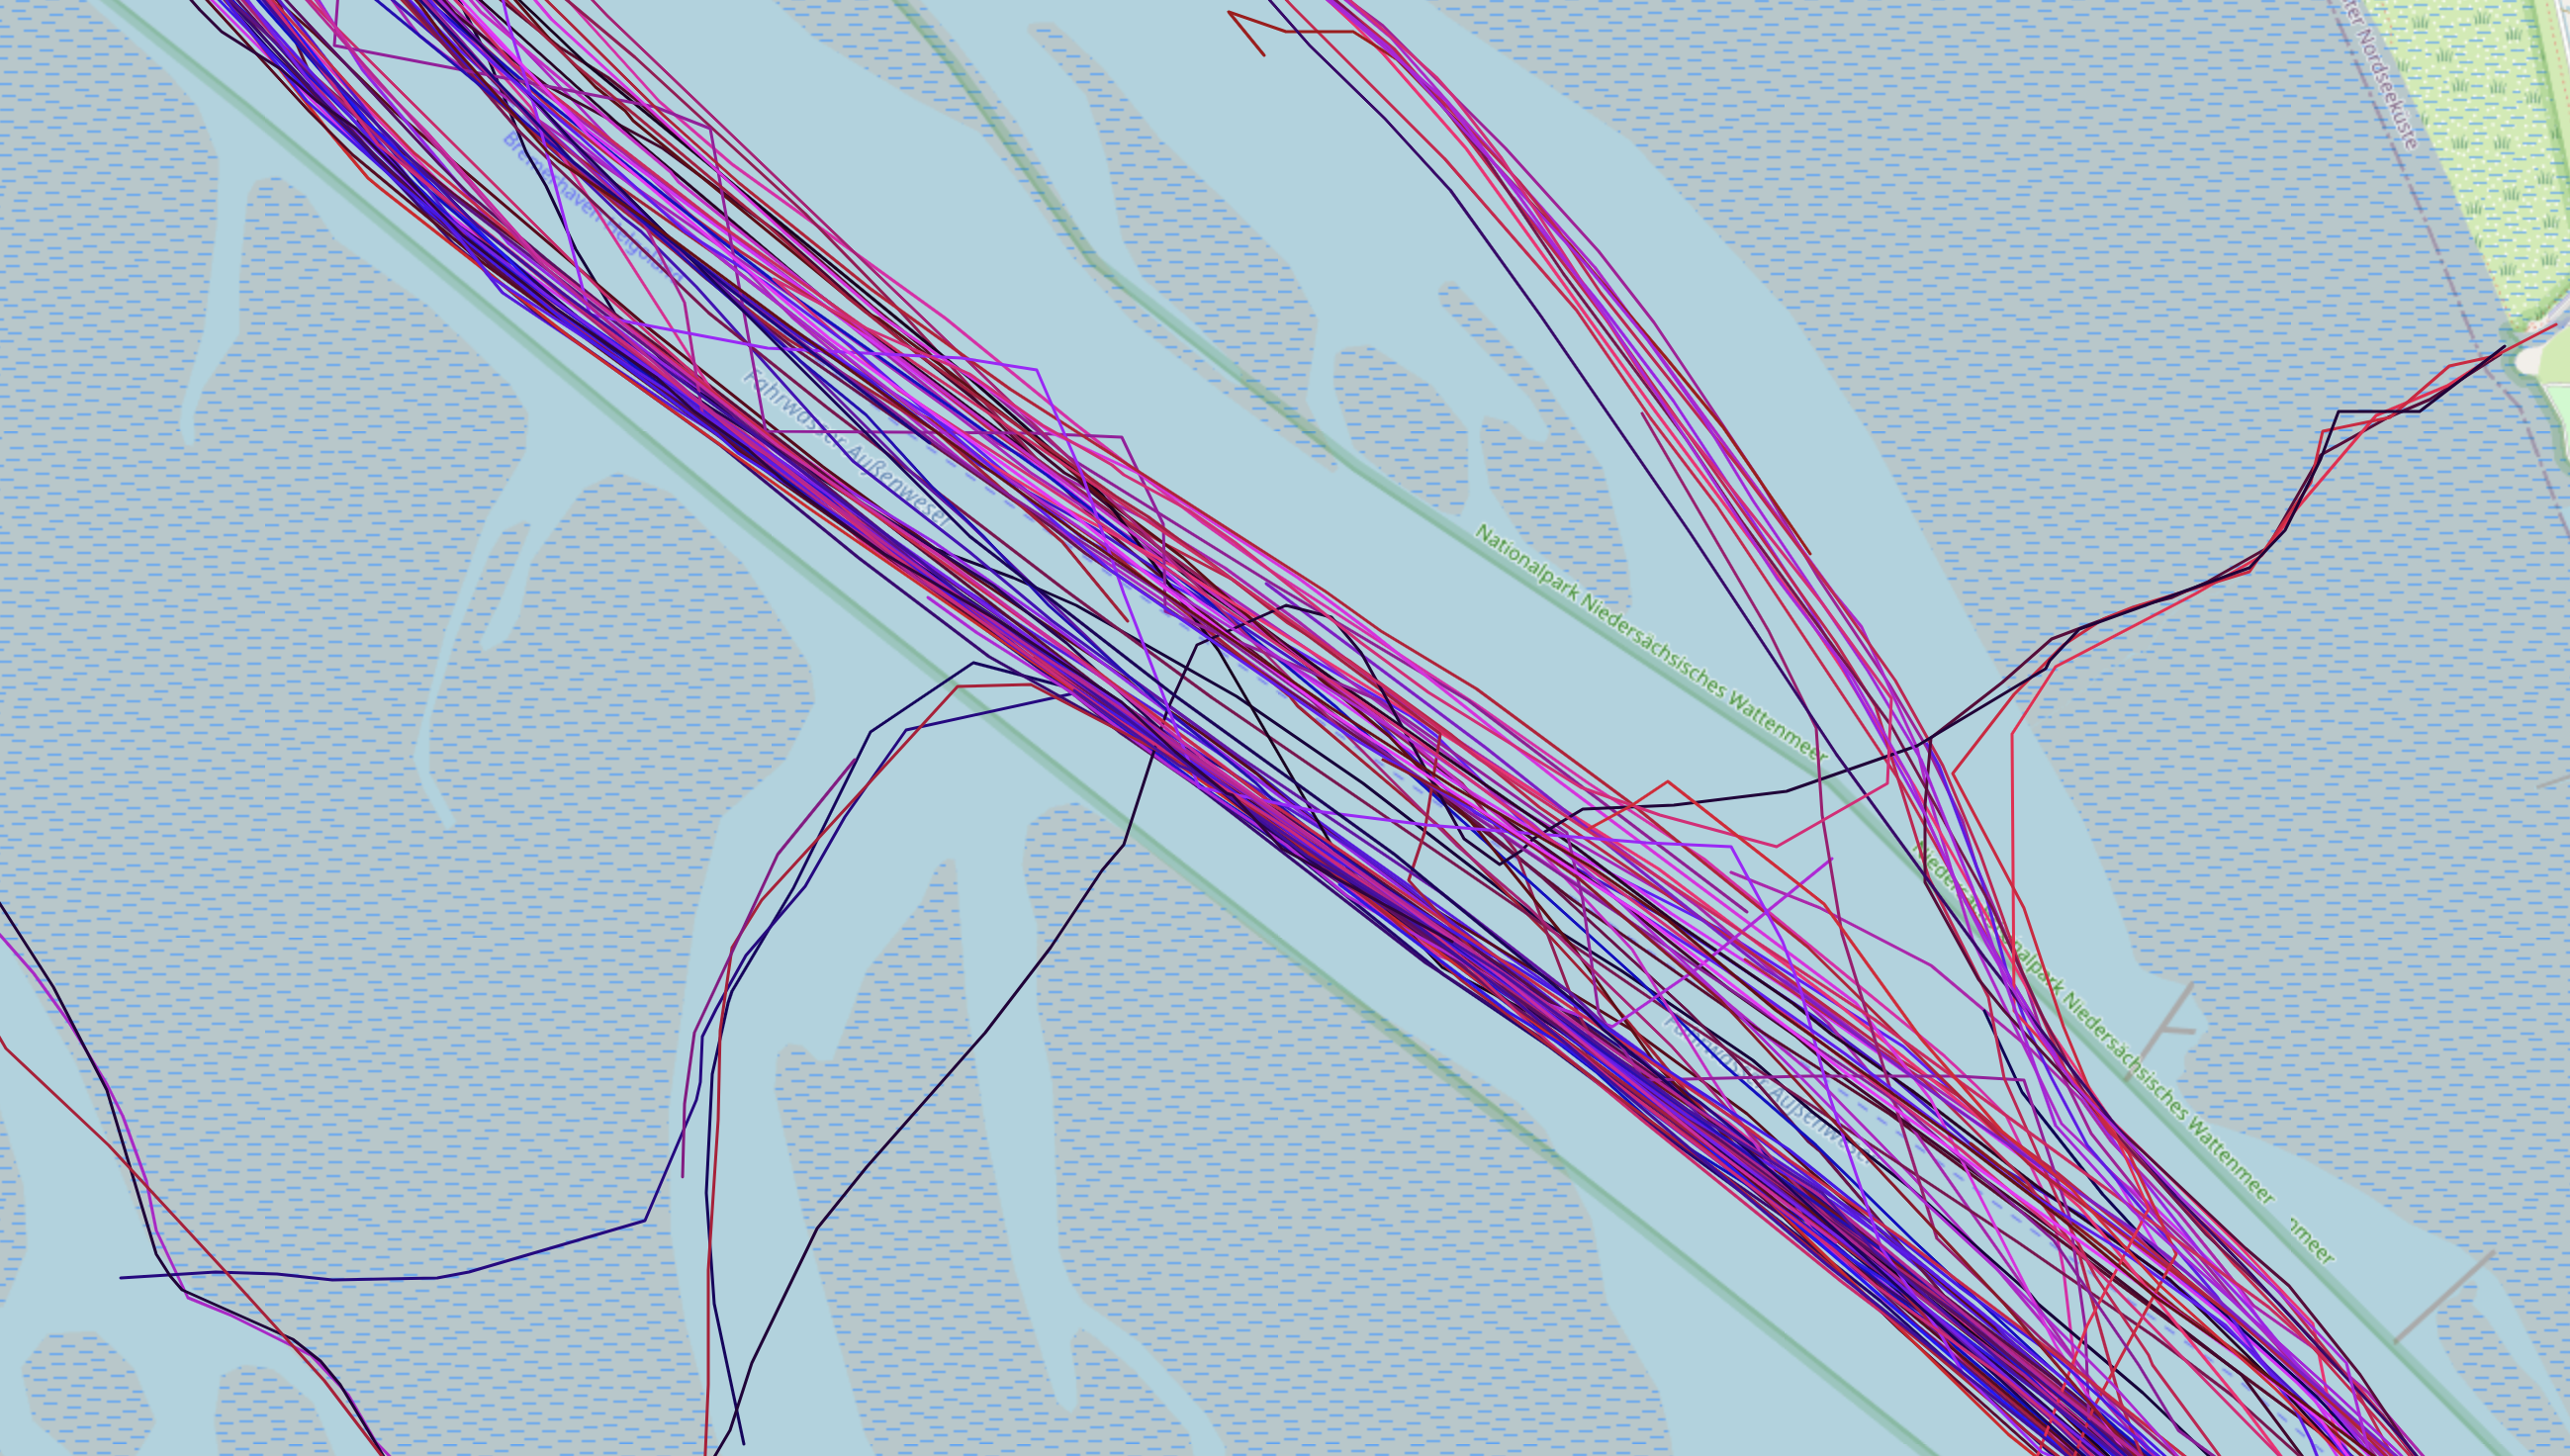
\includegraphics[width=0.48\textwidth]{images/ais/tracks/Sailing.png}
    \caption{Voyages of sailing ships.}
    \label{fig:sailing}
\end{wrapfigure}
Here, we do not split by distinct types, but rather a group of types. The first deviation from the dataset which we call "big ships" focuses on a big variety of different ship models including e.g., cargo- and passenger ships, dredgers, and tanker.
In contrast to the original dataset, ship types that are very dissimilar in terms of propulsion or tend to conduct rapid turning maneuvers get filtered out. Examples for those kinds of ship types are sailing ships and tugs. Recorded trajectories from sailing ships displayed in Fig. \ref{fig:sailing} reveal meandering behavior and unique tracks in shallow fairway that significantly differ from those of cargo ships or tankers.

\begin{wrapfigure}{r}{0.5\textwidth}
    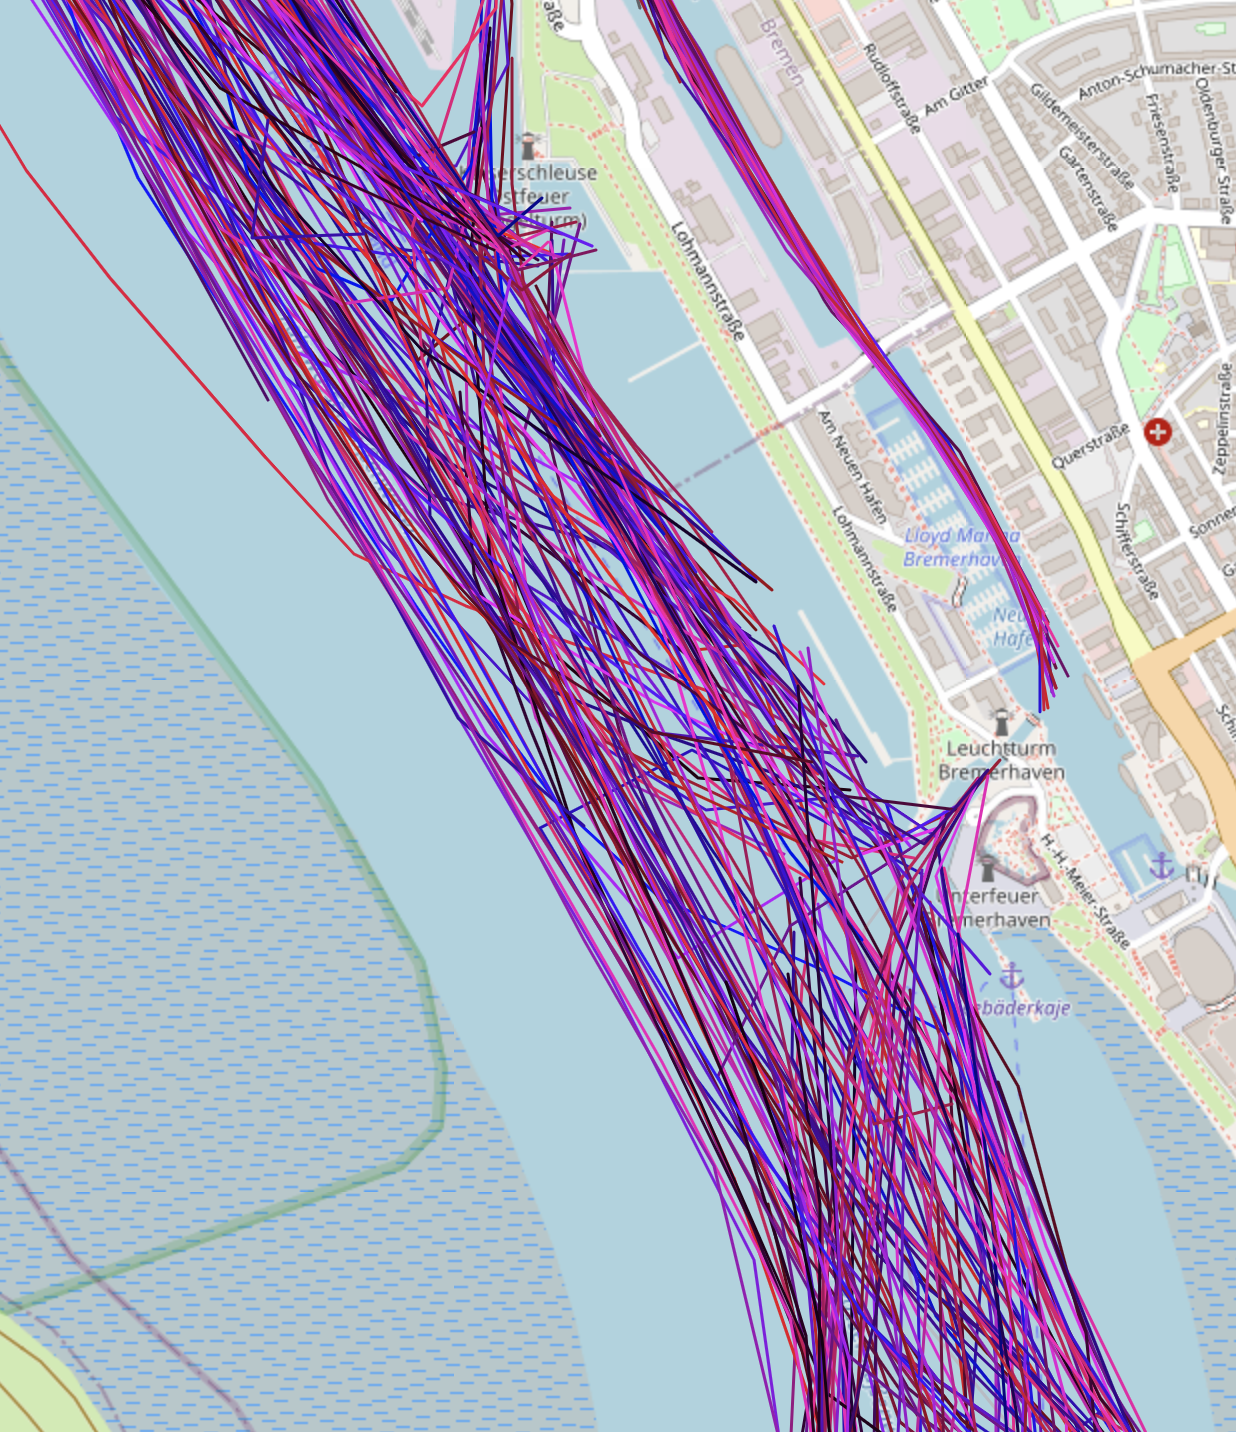
\includegraphics[width=0.48\textwidth]{images/ais/tracks/Tugs.png}
    \caption{Voyages of tugs.}
    \label{fig:tugs}
\end{wrapfigure}
Additionally, (//TODO how much) AIS signals are sent out by tugs which are exceptionally agile, resulting in fast changes to direction and speed as well as quick turns that are visually noticeable in Fig. \ref{fig:tugs}. Although, the filtered dataset "big ships" is shrunk by half, we still expect better results when learning representative trajectories for the reason that the paths themselves are more homogeneous and consistent regarding the sequences of controls (see Fig. \ref{fig:cargoAndBig}). The same applies to the construction of two supplementary datasets that pivot ships that are meant for transportation ("cargo") and ships that carry oil, chemicals or any other fluid or gas ("tanker"). A detailed list of discrete ship types (defined by \textit{myshiptracking.com}) for every category can be discovered in the appendix in section \ref{appendix:datasets}.
\par
The "tanker"-dataset is the most restricted and therefore homogeneous dataset assembled. Fig. \ref{fig:tankerTracks} gives a brief overview of included voyages and their course.
\begin{figure}[H]
    \centering
    \begin{minipage}{.45\linewidth}
            \begin{subfigure}[t]{.9\linewidth}
                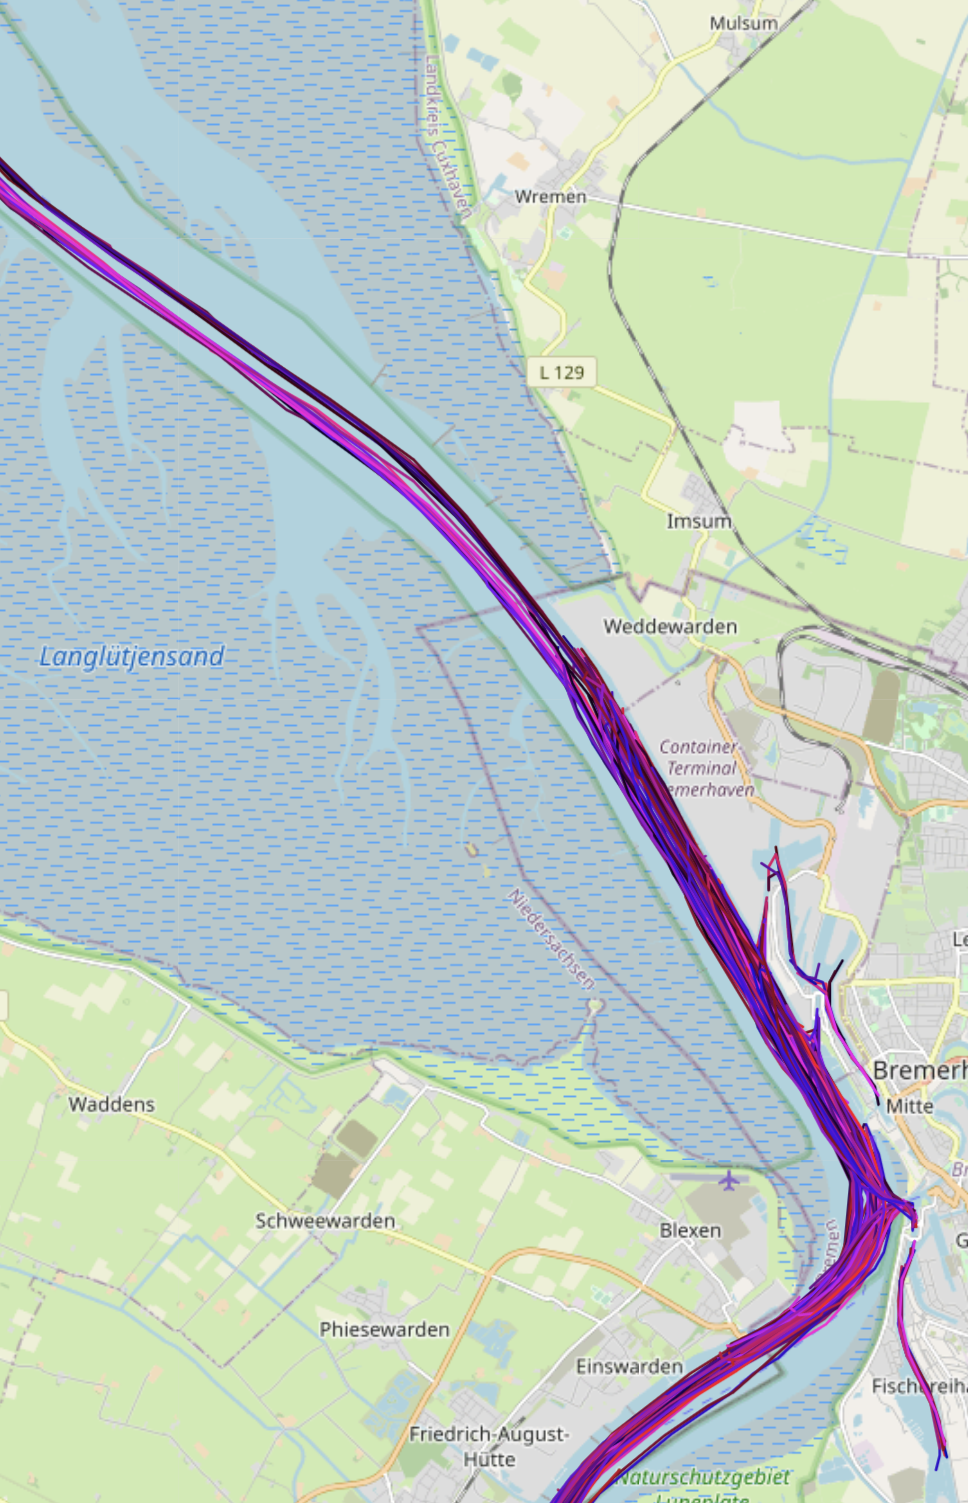
\includegraphics[width=\textwidth]{images/ais/tracks/tanker.png}
                \caption{300 example voyages}
                \label{fig:tankerOverview}
            \end{subfigure}
        \end{minipage}
    \begin{minipage}{.45\linewidth}
        \begin{subfigure}[t]{.9\linewidth}
            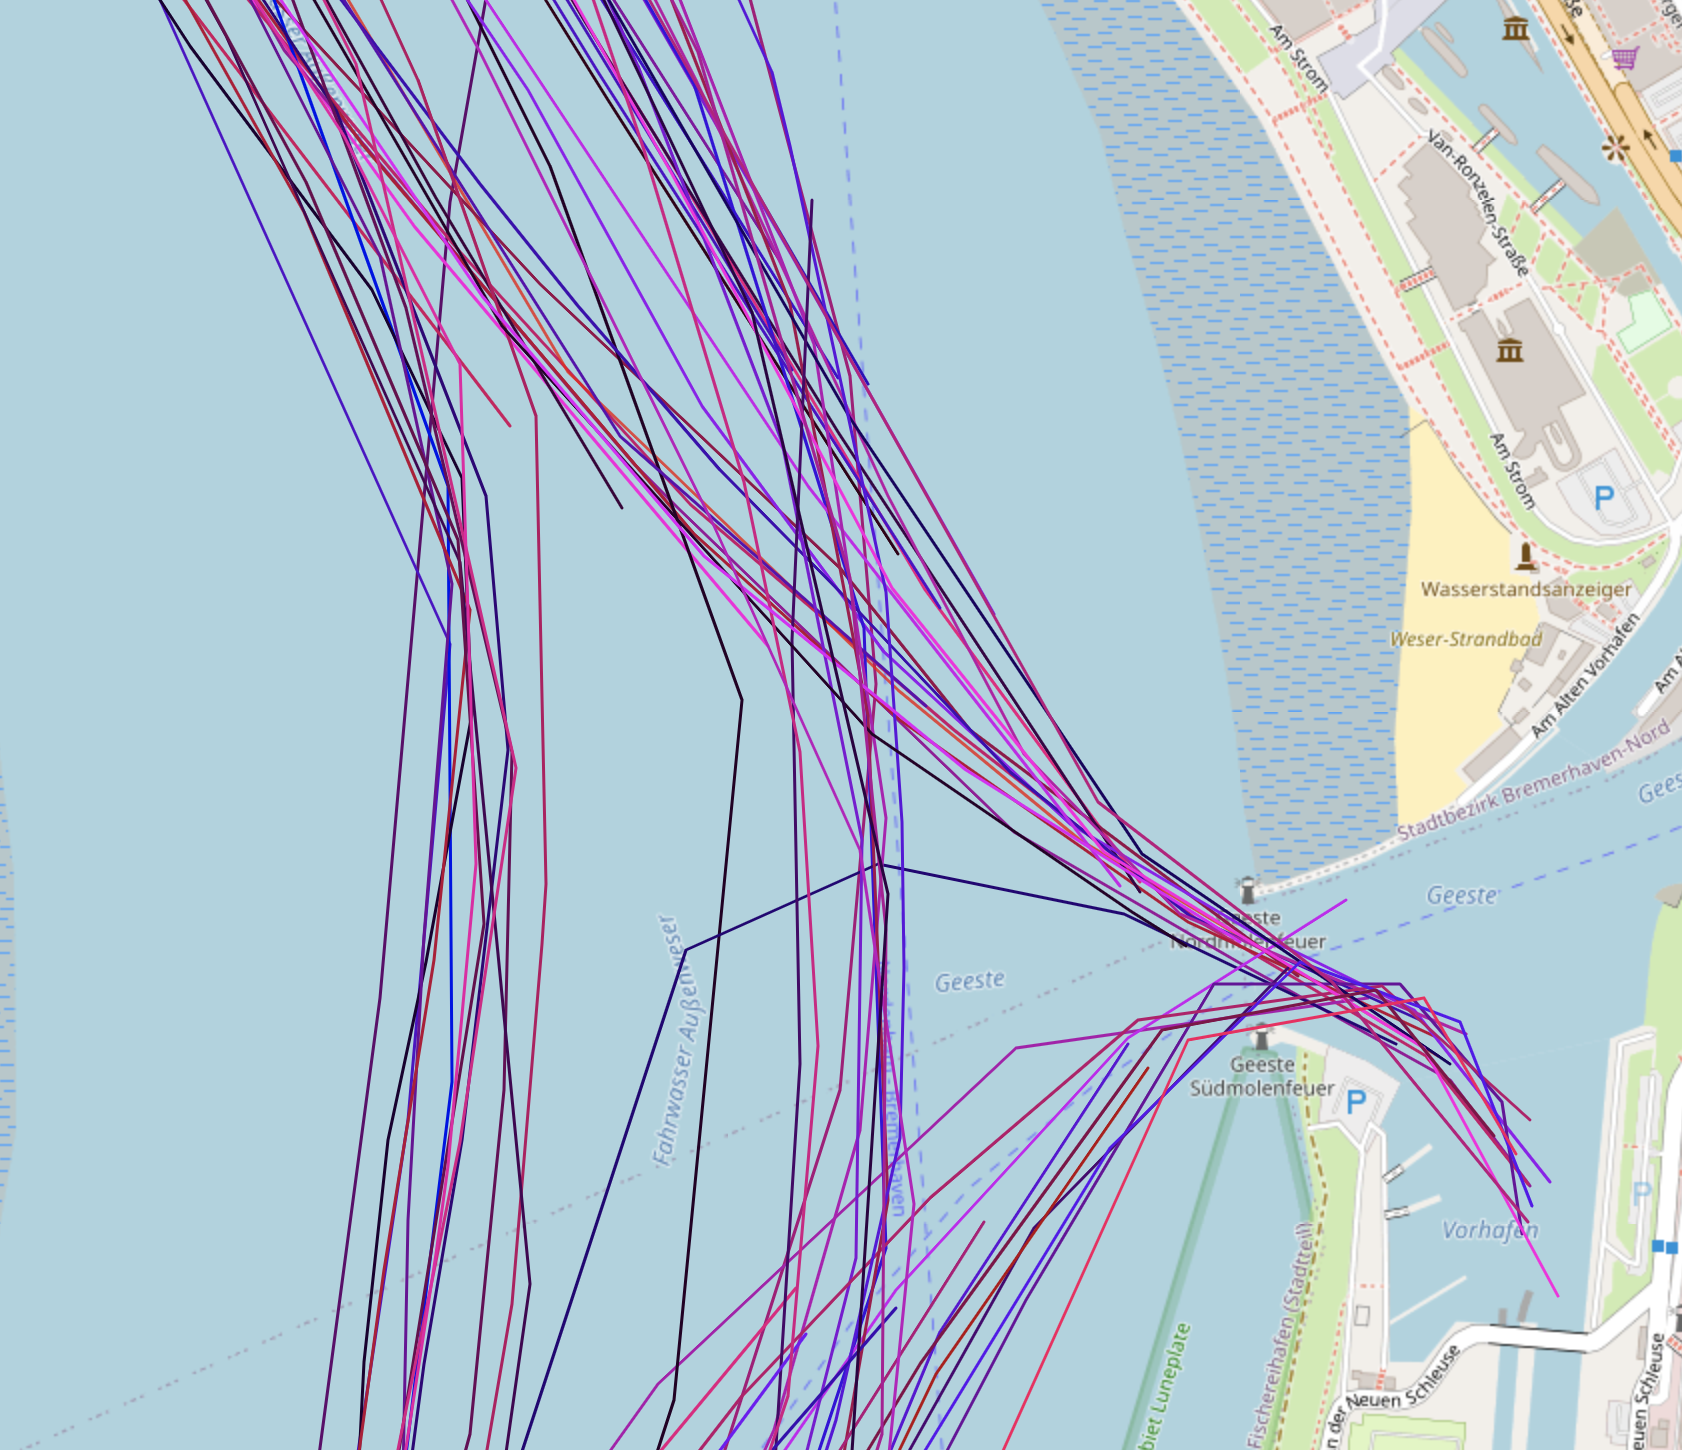
\includegraphics[width=\textwidth]{images/ais/tracks/tanker_partial.png}
            \caption{Entering harbour}
            \label{fig:tankerEntering}
        \end{subfigure} \\
        \begin{subfigure}[b]{.9\linewidth}
            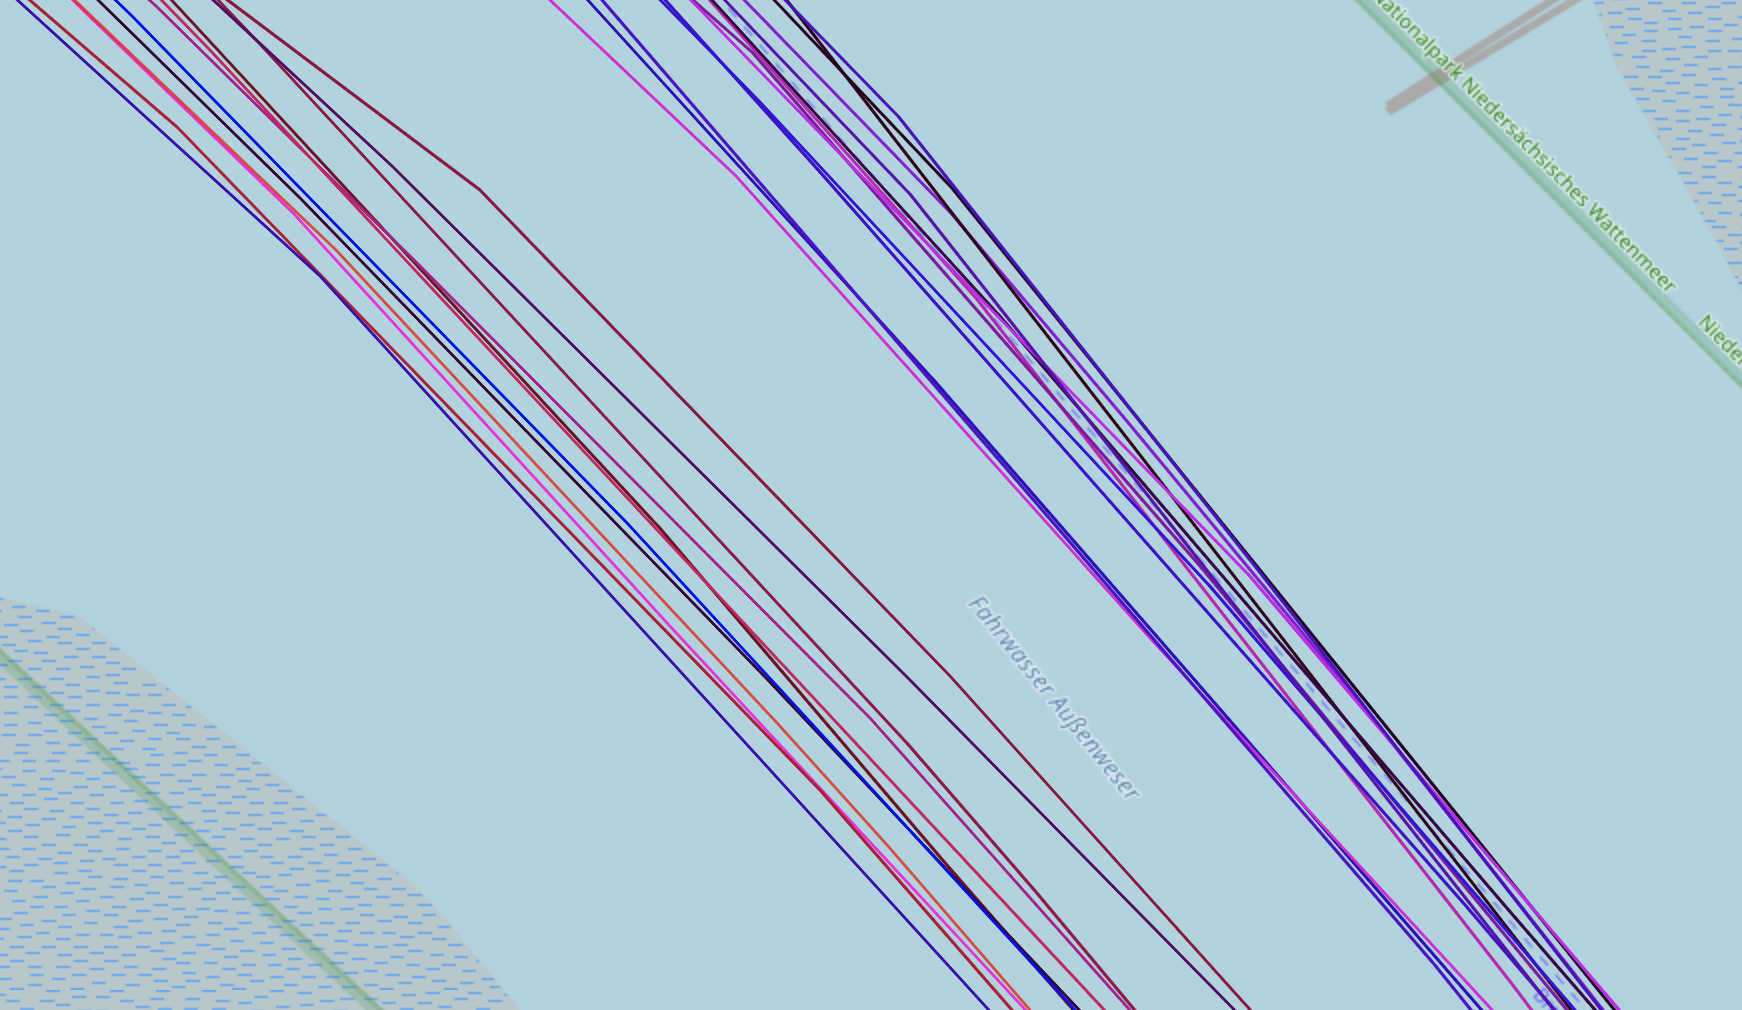
\includegraphics[width=\textwidth]{images/ais/tracks/tanker_fahrrinnen.png}
            \caption{Waterways}
            \label{fig:tankerWaterway}
        \end{subfigure} 
    \end{minipage}
    \caption{Overview of the "tanker"-dataset.}
    \label{fig:tankerTracks}
\end{figure}
Overall, the paths are very clear, meaning that they do not include sudden turns. Furthermore, no obvious outliers can be discovered and ships moving responsively in their respective waterways as shown in \ref{fig:tankerWaterway}.

\begin{figure}[H]
     \centering
     \begin{subfigure}[b]{0.48\textwidth}
         \centering
        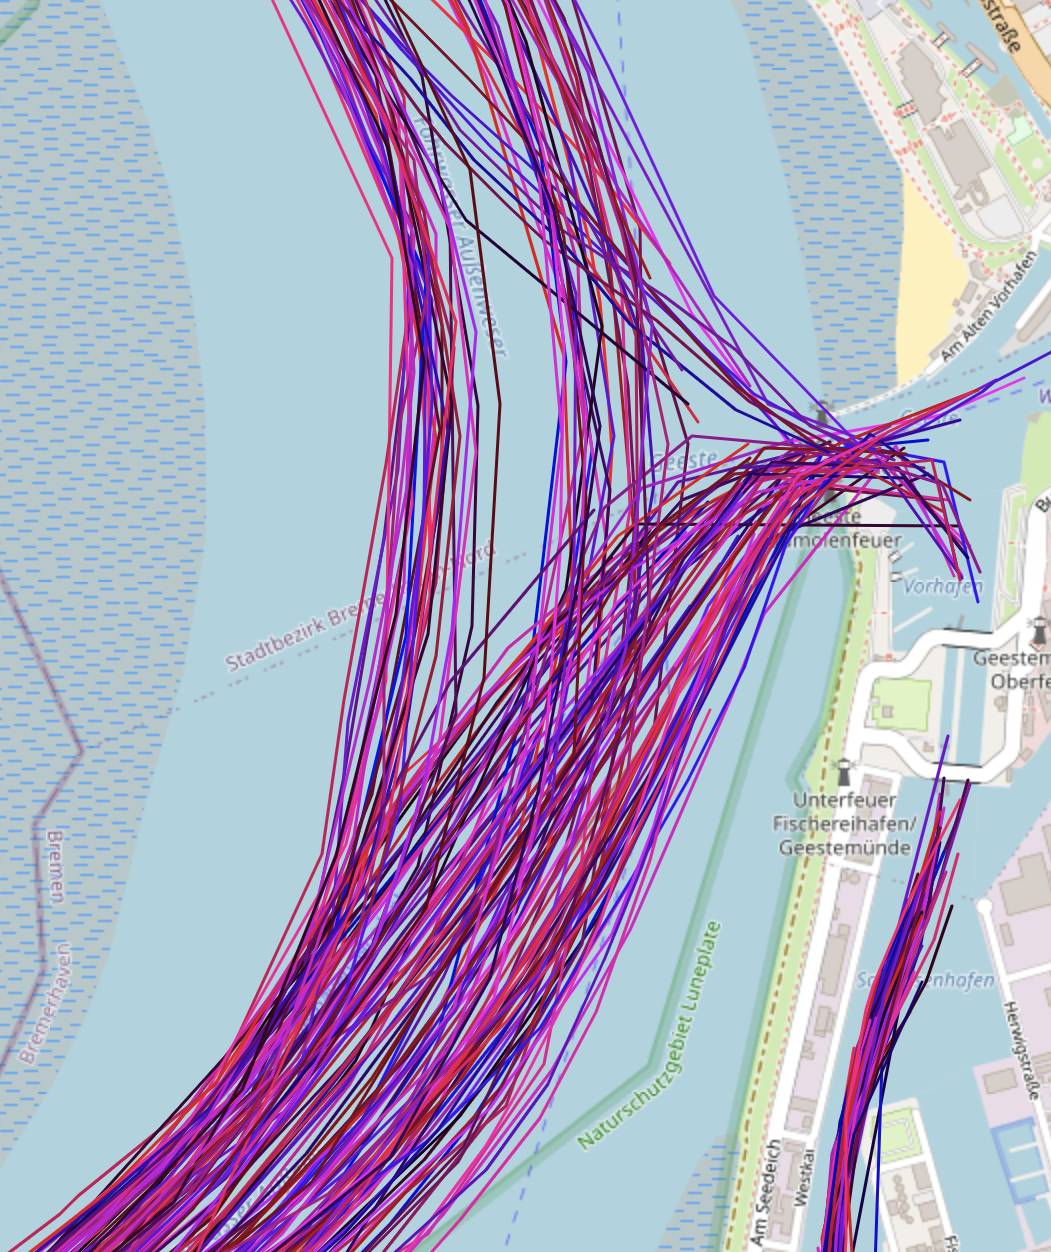
\includegraphics[width=\textwidth]{images/ais/tracks/cargo_entering_fary.png}
         \caption{Subset of "cargo"-ships entering the harbour}
     \end{subfigure}
     \hfill
     \begin{subfigure}[b]{0.48\textwidth}
         \centering
            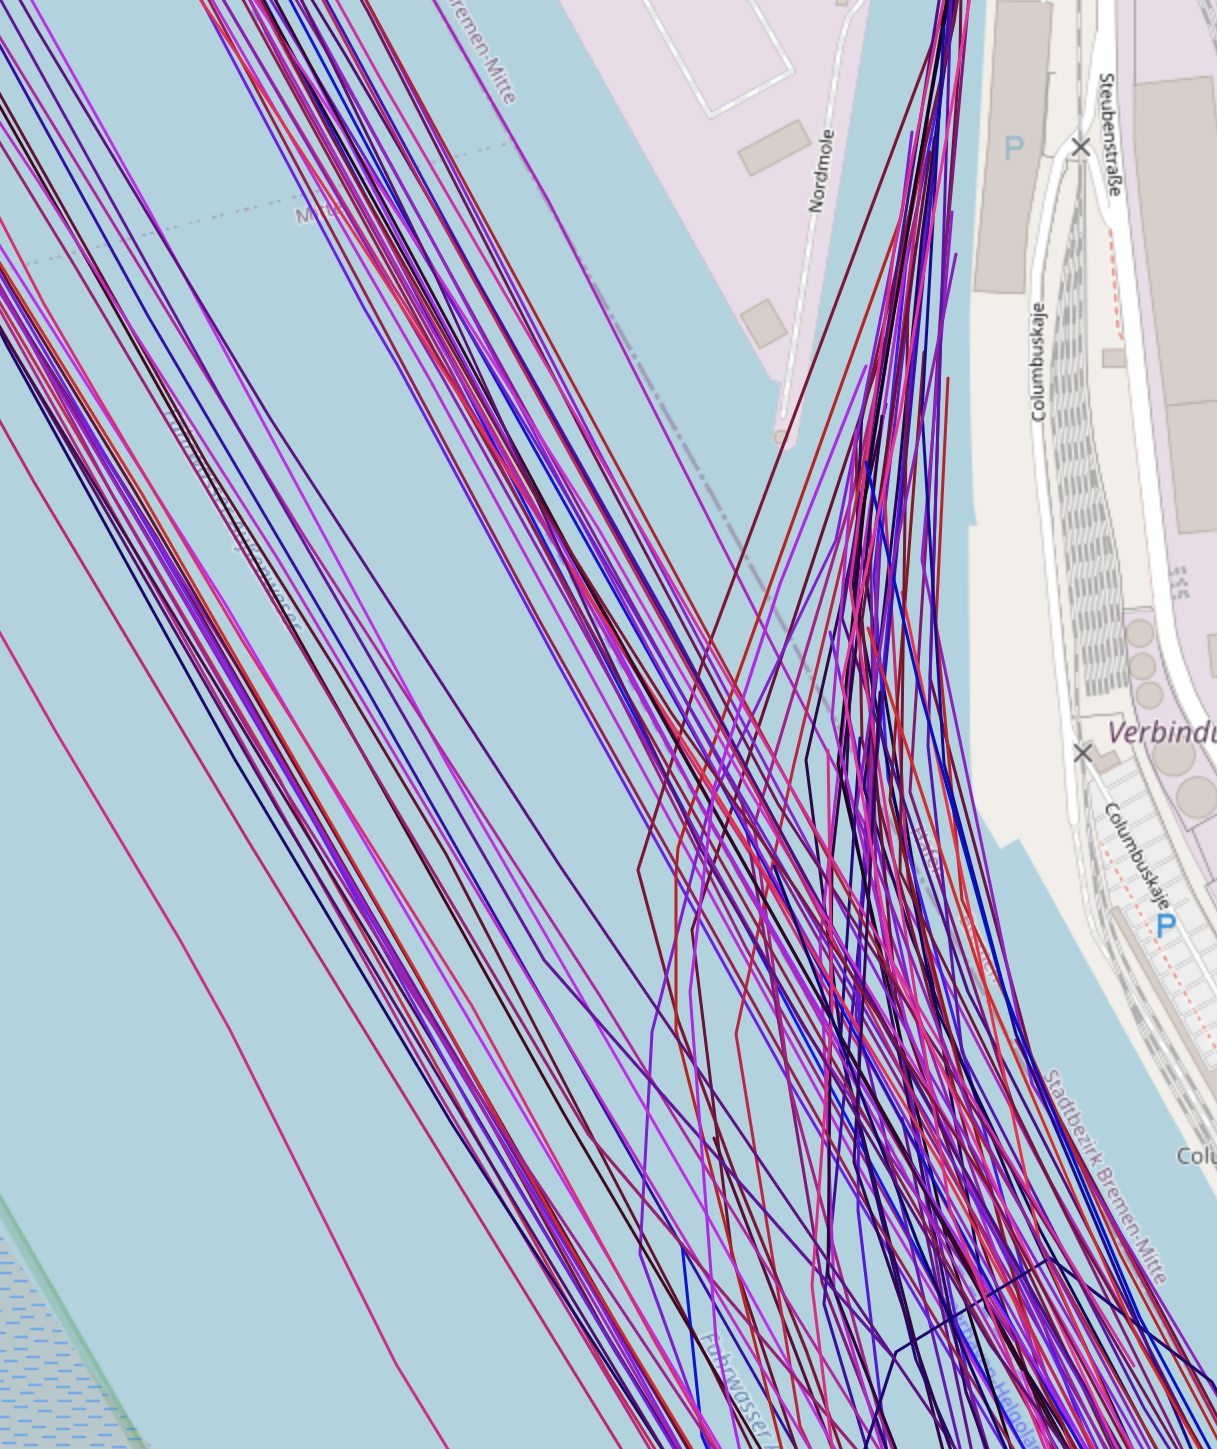
\includegraphics[width=\textwidth]{images/ais/tracks/big_ships_entering.png}
         \caption{Example of "big ships" voyages}
     \end{subfigure}
     \caption{Display of resulting maneuvers from different datasets.}
     \label{fig:cargoAndBig}
\end{figure}


The relationship and amount of unique ships (MMSIs) and extracted trajectories for each of those composed datasets are shown in upcoming Fig. \ref{fig:datasets}, whereas each set is split by 0.85 in training and test trajectories.
\begin{figure}[H]
    \centering
    \hspace*{1cm}%
    \begin{tikzpicture}[node distance=3cm]
    
\tikzstyle{box} = [rectangle, rounded corners, minimum width=4cm, minimum height=1cm,draw=black, text centered, align=center]
\tikzstyle{arrow} = [thick,->,>=stealth]

\node (all) [box] {$\begin{gathered} \textbf{All Ships} \\ \text{MMSIs: 1522} \\ \text{Count: 25019} \end{gathered}$};
\node (big) [box, below of=all] {$\begin{gathered} \textbf{Big Ships} \\ \text{MMSIs: 1077} \\ \text{Count: 11578} \end{gathered}$};
\node (cargo) [box, below left of=big, yshift=-0.5cm, xshift=-1cm] {$\begin{gathered} \textbf{Cargo} \\ \text{MMSIs: 967} \\ \text{Count: 3956} \end{gathered}$};
\node (tanker) [box, below right of=big, yshift=-0.5cm, xshift=1cm] {$\begin{gathered} \textbf{Tanker} \\ \text{MMSIs: 71} \\ \text{Count: 1194} \end{gathered}$};


\draw [arrow] (all) -- (big);
\draw [arrow] (big) -- (cargo);
\draw [arrow] (big) -- (tanker);

\end{tikzpicture}
    \caption{Different datasets and their respective amount of extracted trajectories.}
    \label{fig:datasets}
\end{figure}







